\documentclass{article}

% if you need to pass options to natbib, use, e.g.:
% \PassOptionsToPackage{numbers, compress}{natbib}
% before loading nips_2016
%
% to avoid loading the natbib package, add option nonatbib:
% \usepackage[nonatbib]{nips_2016}

\usepackage[final]{nips_2016}

% to compile a camera-ready version, add the [final] option, e.g.:
% \usepackage[final]{nips_2016}

\usepackage[utf8]{inputenc} % allow utf-8 input
\usepackage[T1]{fontenc}    % use 8-bit T1 fonts
\usepackage{hyperref}       % hyperlinks
\usepackage{url}            % simple URL typesetting
\usepackage{booktabs}       % professional-quality tables
\usepackage{amsfonts}       % blackboard math symbols
\usepackage{nicefrac}       % compact symbols for 1/2, etc.
\usepackage{microtype}      % microtypography
\usepackage{xcolor, graphicx, subcaption, float, enumitem, amsmath}

\newcommand{\selfnote}[1]{\footnote{\textcolor{red}{#1}}}
\newcommand{\domainDoubt}[1]{\footnote{\textcolor{teal}{#1}}}
\newcommand{\technicalDoubt}[1]{\footnote{\textcolor{blue}{#1}}}

\title{Commuter classification and behavior clustering: Beijing use case}

% The \author macro works with any number of authors. There are two
% commands used to separate the names and addresses of multiple
% authors: \And and \AND.
%
% Using \And between authors leaves it to LaTeX to determine where to
% break the lines. Using \AND forces a line break at that point. So,
% if LaTeX puts 3 of 4 authors names on the first line, and the last
% on the second line, try using \AND instead of \And before the third
% author name.

\author{
  Selene Baez  Santamaria \\
  \texttt{s.baezsantamaria@student.vu.nl}
}

\begin{document}
% \nipsfinalcopy is no longer used

\maketitle

\begin{abstract}
  Public transportation, centered on subway and bus networks, is an data-rich domain that can benefit from data mining and machine learning techniques. The classification of commuters versus non-commuters/occasional travelers can help government, transport management and operators to better target their policies in order to improve the transportation network in large cities. Furthermore, characterizing commuters by behavior clustering can bring deeper insight into their needs and routines as a whole. 
  This project proposes the usage of ensemble models for classification and clustering of public transport users. For this purpose, transit card data will be used, available from the city of Beijing, China. 
\end{abstract}

\newpage

\tableofcontents

\newpage
\section{Introduction}

\subsection{Urban public transportation}
% Why is public transportation important?
Urban public transportation includes systems that are available for use by anyone in urban areas. Its facilities are commonly composed by buses, subway/metro lines, light rails, tramways, trains, taxis and others. As a network, they provide service for the majority of citizens in urban areas.\citep{vuchic1900urban}

Figure \ref{fig:transportation/passenger} shows the passsenger transport usage, as million passengers per kilometer, in several different countries according to the Organisation for Economic Cooperation and Development (OECD). From all OECD countries, the United States, China, Germany, France, Italy, and the United Kingdom contitute the six countries with the most passenger transport, according to their reported data from 2015 or later.\cite{OECD2017passenger} 

\begin{figure}[H]
  	\centering
  	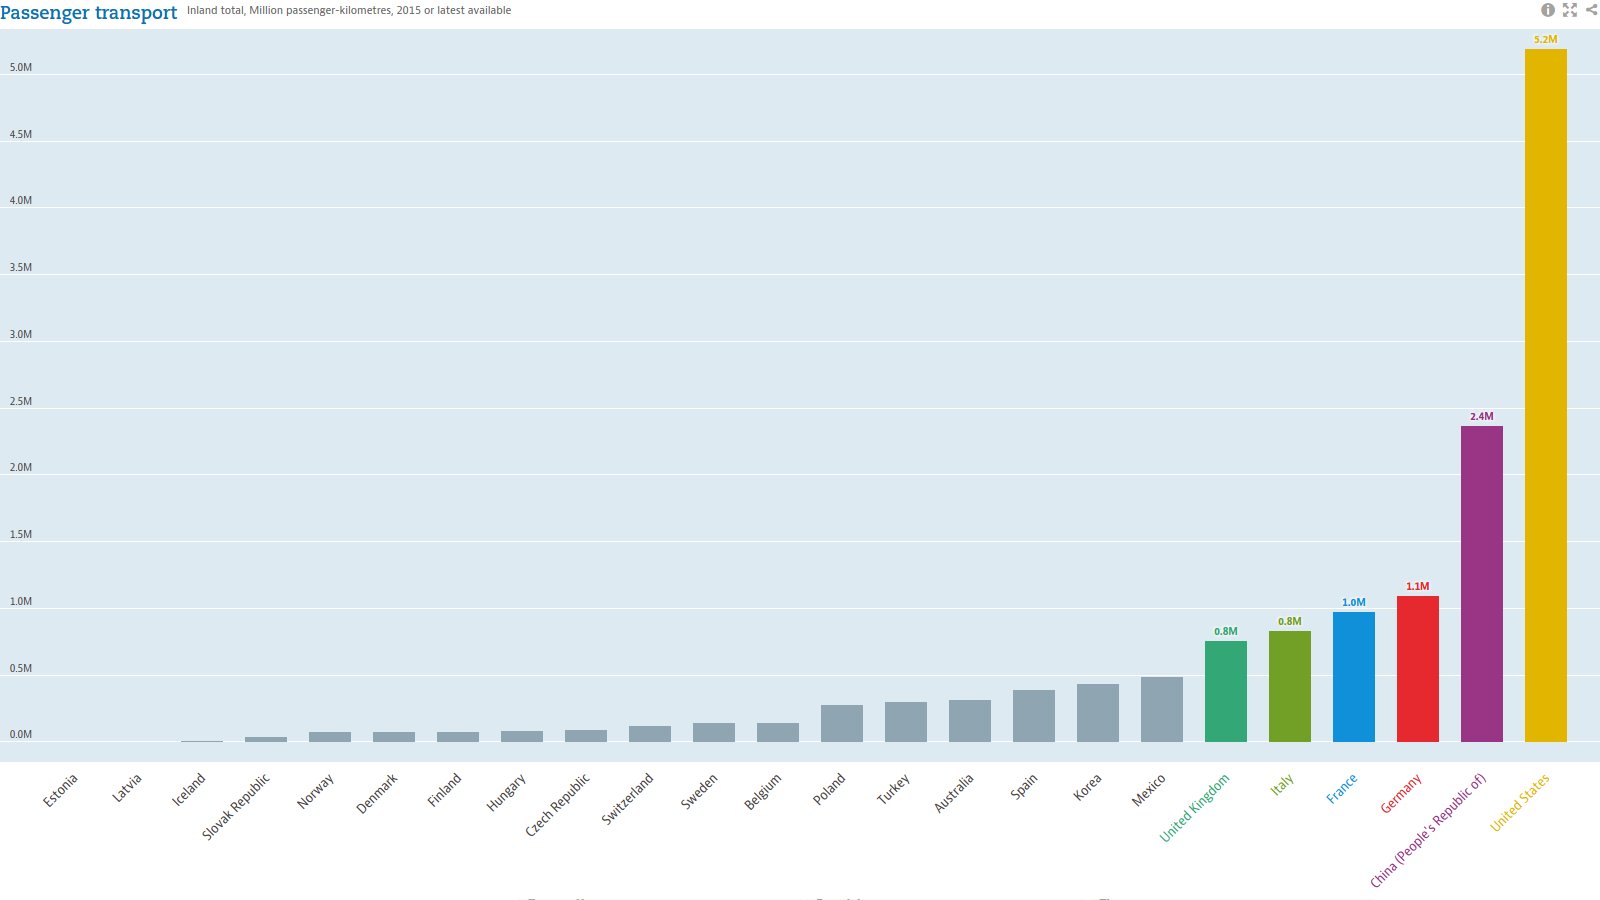
\includegraphics[width=\linewidth]{./images/OECD_passengers_absolute.png}
  	\caption{OECD countries and their passenger transportation data.}
  	\label{fig:transportation/passenger}
\end{figure}

Furthermore, historical data in Figure \ref{fig:transportation/passenger-trend} reveals the 15 years behavior for each of the aforementioned countries. Most of the countries show stability, with increase or decrease of less than 0.10 million passengers for European countries, and 0.5 million passengers for the United States. China, however, shows a trend with steep increase for most of the selected years. In fact, comparing to its less than 1.2 million passengers in 2000, China doubled its public transport usage to 2.4 million passengers in 2015. 
  
\begin{figure}
  	\centering
  	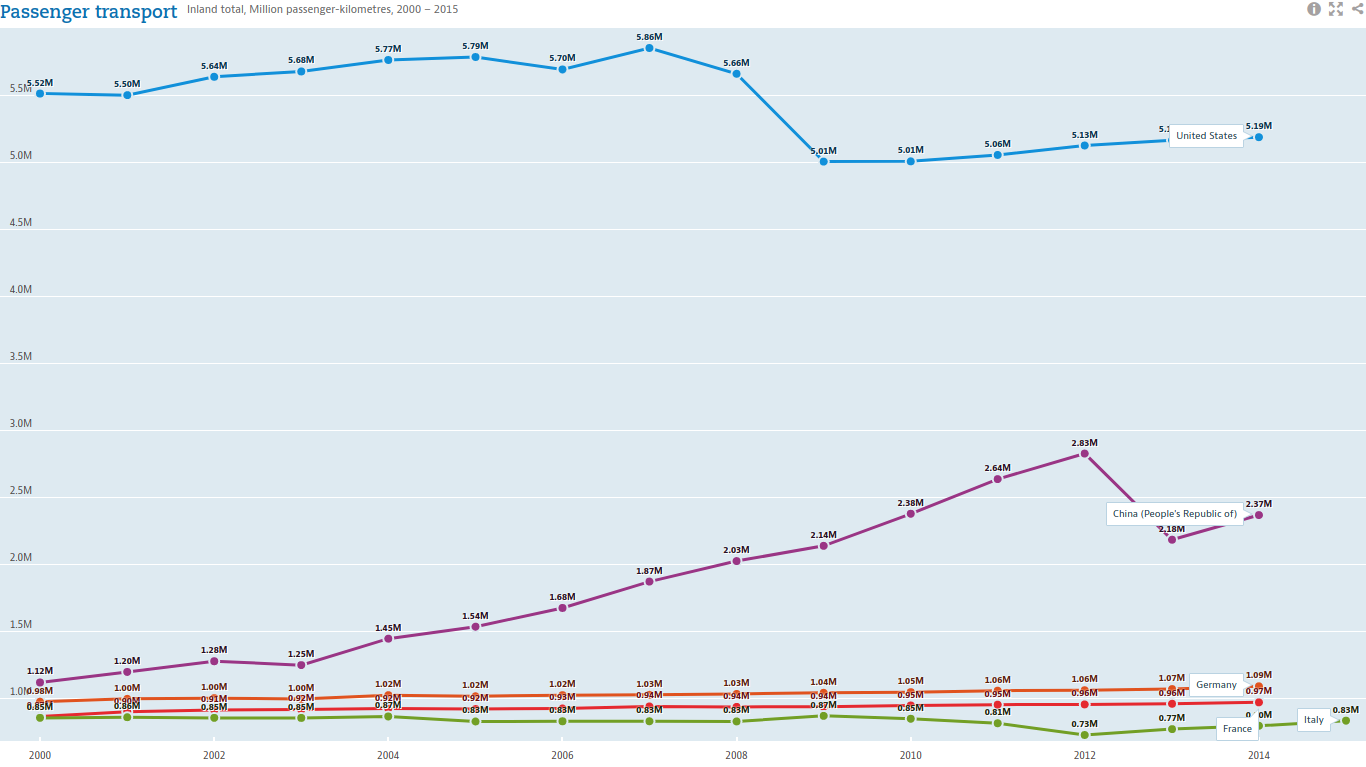
\includegraphics[width=\linewidth]{./images/OECD_passengers_increase.png}
  	\caption{Historical data for the top six countries with most passenger transport usage. China (top-left image) has the steepest increase overall.}
  	\label{fig:transportation/passenger-trend}
\end{figure}

Though it is a more sustainable alternative compared to private car usage, public transport usage has a significant environmental impact, affecting noise and air pollution. Diesel buses, which generally make up a major part of public buses, have large fuel consumption needs and contribute significantly to CO$_{2}$ emissions. Even eco-friendly alternatives such as hybrid diesel buses are sensitive to operating conditions, as their fuel consumption may increase by up tp 50\% when the on-board air conditioning is on.\cite{zhang2014real}

Consequently, public transportation directly relates to energetic demand, since its facilities are mostly petroleum or electrical based. In terms of global energy consumption, passenger transportation accounts for about 25\% of the total world energy consumption. Furthermore, the transportation sector consupmtion increases at an annual average rate of 1.4.\% \cite{eia2016energy} This may bring further economical implications for countries with high public transportation demand.

\subsubsection{Who are the commuters?}
% Self proclaimed commuters
A major proportion of public transport users is represented by commuters. These are regular users of public transit, with consistent spatiotemporal patterns in their travels. Driven by a routine, commuters travel back and forth from specific places, for example, from their home to work, school, or other similar locations. 

As commuters are frequent users of public transit, the  conditions of the public network directly influence their personal well being and generally impact their quality of life. Intuitively, if the commuting experience is unpleasant, daily travel can bring distress to commuters and/or even repel them from using the public transport at all. Several studies have looked into public transit evaluation from different perspectives, including commuters' needs \cite{mao2016commuting}. The most common aspects of it include: travel time, average speed, delays, accessibility, service coverage, crowded level, facilities quality, and fare rate. Weng et al \cite{weng2013bus} identified five indexes (Convenience, Rapid, Reliability and Comfort) that summarize commuters priorities when choosing to travel by public transport.
 
From both of the above, the large presence of commuters and their known needs and preferences, it follows that identifying commuters and addressing their needs can help in creating a sustainable public transportation network. Public transit stakeholders should be able to understand the commuters' demands and its dynamics, consequently bringing long term planning and policies for improving the overall commuting experience.

\subsection{The city of Beijing}
% Why is beijing a good (challenging, rich, valuable, relevant) use case?
The city of Beijing presents a special case of urbanization and rapid industrialization. This is reflected in a sudden population growth of 20\% per decade since 1960, with the largest increase of 44\% in the last ten years. The latest official census in 2010 reported the urban agglomeration of Beijing (including Beijing itself and its adjacent suburban areas) having a population of 19,612,368 people. The UN World Urbanization Prospects estimates the 2017 population at over 22 million inhabitants. \cite{world2016beijing}

As a result of the population explosion, many environmental and social resources are under pressure. From the environmental side, one of the most notable issues is related to air pollution, due to the significantly high pollutant emissions in the city \cite{zhang2016air}. Similarly, the city's downstream river pollution is serious, with most regions of the Yellow river being unable to comply with the lowest water quality standards. \cite{wang2015studies} 

On the aspect of social resources, one of the main complications is mobility. In Beijing, public transport is the dominant mode of transportation, accounted for 44.0\% of all trips compared to 32.6\% attributed to private cars \cite{mao2016commuting}. In 2008, the total ridership was 6.5 billion travels. Though the network is continually expanding, it is a fact that public transport is overcrowded, constantly reaching over 100\% capacity \cite{beijing2009research}.

Beijing public transport is composed of buses, subway and bicycles. The three types can be accessed by using a single smart card. 

\begin{description}
\item[Bus:] In 2015, there were 876 bus lines with 23,287 buses in operation. The bus network is the most extensive mode of transportation, expanding over 20,186 km. It observes an average daily traffic volume of 10.98 million passengers, with the highest daily volume reaching 13.07 million on one day. \cite{beijing2016annual}

\item[Subway:] The Beijing subway has 18 lines with 334 stations, of which 53 are transfer stations. In 2015 it had an operating length of 554 km, with 5,024 vehicles running. \cite{beijing2016annual} Its network is split by two operators: the state-owned Beijing Mass Transit Railway Operation Corp (operating 15 lines), and the joint Hong Kong venture Beijing MTR Corp (operating 3 lines).

Beijing's subway has an average daily traffic volume of 9.11 million passengers, with a maximum recorded volume of 11.66 million passengers. As such, it is the second busiest metro system in the world, providing 3,410 million annual journeys. Compared to the service provided in 2012, the system observed a 39\% increase in usage by 2014. It is also the second longest metro network, surpassed by Shanghai by only 21 km.  \cite{uitp2015world} 

\item[Bicycles:] Beijing first implemented public bicycle systems in 2012. As of 2015, in total, 67,000 bikes are available for rental with 2,700 pick up/drop off points spread across the city. \cite{beijing2016annual}
\end{description}


\subsection{Smart cards and Big Data}
Smart cards present us with a straightforward way of massively collecting daily data. In the last years, smart card systems have become more popular in the Transportation domain, making it possible to monitor travelers transactions and facilitating fare collection. Several cities have implemented such systems, for example the Octopus card in Hong Kong\cite{chau2003octopus}, Oyster card in London \cite{blythe2004improving}, OV-chipkaart in The Netherlands \cite{de2008analysis}, and Yikatong card in Beijing \cite{chan2010tactical}, to name a few.

In Beijing, over 90\% of public transit users are smart card holders. There is a significant incentive for using the Yikatong smart card since bus rides are heavily subsidized (users have only to pay 50\% of the full price)\cite{ma2017understanding}. Moreover, the Yikatong smart card system is also integrated with taxi, electricity and sewage payments, making it convenient to use as a general paying method.

\paragraph{Data quantity}

Placed in context, public transit systems serve at least hundreds of users daily, where a typical user performs several trips a day, every day. On the specific case of Beijing, there are hundreds of thousands of smart cards gathering between 5 and 16 million records (trips) a day, among a large complex network containing thousands of routes and tens of thousands of stops. 

\paragraph{Data quality}

However, though smart cards exponentially increase the quantity of data, they do not completely guarantee its quality. As is, some aspects of the trips cannot always be faithfully recorded but are inferred (for example, the transfers between the subway system when no check-in/out is done at changing trains). Furthermore, some fields are sometimes simply missing or incorrectly recorded due to malfunctions and situations out of control. 


Given the large amounts of data collected and its nature, the analysis of such becomes challenging. Transit smart cards are capable of recording spatiotemporal information at an individual level over long periods of time. This generates a large volume of historical data that only tailored big data techniques can deal with. 

\subsection{Project motivation}
This project performs an interdisciplinary study between the areas of Artificial Intelligence and Metropolitan Transportation. It is focused on introducing data mining techniques to a data rich domain. 

% Each science benefits
The area of Artificial Intelligence is able to provide dozens of prediction algorithms. Though constantly under refinement, it is time for state-of-the-art techniques to be applied, tested and validated under real and large impact situations to test their ability to deal with noisy streams. Comparably, given the ever growing complexity of urban mobility, domain experts must focus on analyzing trends and insights instead of curating and making sense out of raw data. As such, introducing these state-of-the-art techniques into the Metropolitan Transportation domain can aid to unravel massive human behaviors and reveal patterns and trends in mobility.

\subsubsection{Societal context}
% description, prediction and preescription
Identifying and analyzing mobility patterns may have different goals, from description, prediction or prescription, all of which affect their stakeholders directly. 

A descriptive analysis determines how people use the public transit. It can pinpoint chaotic hotspots in the city, peak hours, popular routes or other behaviors. A predictive analysis investigates how will people use the transit in the future or under new circumstances. For example, public transport usage projections in the years to come directly affects environmental models trying to improve air and water quality, energetic demand or other natural  and economic resources.

Finally, a prescriptive analysis focuses on how should the different stakeholders deal with mobility behaviors. For example, the government as well as transport management and operators would gain invaluable spatial and temporal insights regarding commuters' behaviors. This insight may lead to tangible results, including policies for increasing the efficiency of the public transit network, adjustable travel fares tailored to the most relevant mobility patterns, incentives to relieve peak hours and thus traffic congestion, urban planning for residential and industrial land use, and others.

Given that Beijing has a widely spread data collection system, combined with formidable institutions capable of introducing new measures in their public transportation network, this city is an excellent use case where the results of an in-depth study can generate actionable plans and bring benefits in the short and long term.

Furthermore, the social context of Beijing presents specific opportunities for improvements where the full power of data analysis and its impact can be tested. For example, the city of Beijing faces a large imbalance between residential and working areas. Due to urban expansion, most residents have been forced to move to suburban areas due to the lack of affordable housing, regardless of having their work environments within the six Ring Roads \cite{zhou2014commuting}. Investigating and targeting this group could alleviate the pitfalls of long distance commuting. 


\subsubsection{Scientific context}
% Improve individual and collective analysis
Mobility patterns in metropolitan areas follow complex swarm behaviors. Based on individual travels and routines, travelers exhibit distinguishable characteristics on a larger scale. Both individual and collective levels of understanding are crucial for Transportation experts. In order to explore both levels, Metropolitan Transportation studies typically focus of the usage of surveys. These surveys are targeted to reach travelers on an individual level, while large scale indicators and aggregated data are taken to investigate their collective behavior. 

These methods have several disadvantages. On the one hand, surveys are costly to implement, and in general have problems related to small non-representative samples. Even when these problems are escaped, the usual quality versus quantity trade off is present, reducing the confidence of the collected information. On the other hand, large scale measurements (i.e. total passenger flow) miss the interactions between individuals that cause the collective behavior.

On top of this, an important consideration on the Metropolitan Transportation domain is that the data collected by smart cards is unlabeled. This means that traveling behaviors are not assigned to known specific categories, making it hard to validate and evaluate. Typically, this issue is address by asking some sample users -via surveys- how they categorize themselves (for example, if they consider themselves to be commuters) and then extrapolating this profile to new users. However, self-reported data by itself has bias problems, therefore introducing noise or false patterns. 

Fortunately, the field of pattern recognition has seen major development in the last years. Nowadays, there exist machine learning and other data mining methods specialized in analyzing disaggregated complex information. Data analysis can be as general is specialized as needed, producing reliable and comprehensible information and visualizations. Furthermore, unsupervised tools have arisen that find patterns based on the data alone, thus being independent from the aforementioned biases.


\subsection{Thesis organization}
The rest of this thesis is organized as follows: On the next section we perform a \textit{Literature review} to explore previous work on mining smart card transit data. We also summarize current representation and pattern recognition methodologies for dealing with complex spatiotemporal data.  

Subsequently, we establish the \textit{Research framework} where we explicitly state the objectives and research questions of this project. As a result, we limit the project's scope and clearly define the most important terms to be used. 

We continue to describe the \textit{Methodology} thoroughly. This consists of an extensive description of the data and its characteristics, our proposed 3 dimensional representation for spatiotemporal data, and the data mining approach to follow, including supervised and unsupervised learning techniques for dimensionality reduction and pattern recognition.

Following this, we identify three distinct stages of the project: \textit{Data preparation and preprocessing}, \textit{Commuters identification}, and \textit{Traveling behavior clustering}. In the \textit{Data preparation and preprocessing} section we describe the pipeline for processing raw data, extracting trip attributes and finally creating the proposed 3D representation of an user's traveling behavior. 

The section on \textit{Commuters identification} describes a supervised learning approach for classifying labeled data, using feature selection and ensemble models. Its counterpart, the section on \textit{Traveling behavior clustering} describes an unsupervised  learning approach to recognize similar traveling behaviors, using feature extraction (by means of an autoencoder) and clustering algorithms. 

Finally, we gather conclusions regarding the proposed representation. We compare both supervised and unsupervised approaches and explore future work opportunities. 

\newpage
\section{Literature review}
In this section we look at studies within the last decade that are related to smart card transit data. First, we summarize the approach and the most relevant findings of each paper in order grasp a broad view of the Transportation domain. Secondly, we explore representations for spatiotemporal data and compare the way traveling behavior is usually represented in the Transportation domain, and other types of representations available in the Artificial Intelligence domain. Thirdly, we discuss techniques for pattern recognition through supervised and unsupervised learning. Finally we explore some pioneer work in end-to-end learning. 

\subsection{Data mining on transit card data}
% What questions and approaches are common. How do they interpret traveling behavior? What's the volume of data?
With the introduction of smart card systems in large cities, several studies have aimed to extract knowledge from the large amounts of data collected. Many of this studies focus on analyzing traveling behavior, which is regarded as a spatiotemporal mobility pattern. Though different in their methodology, results concerning commuters are duplicated across studies. As the spatial and temporal regularity of commuters' travel behavior is evident in their smart card data, they pose an excellent opportunity of study.

Morency et al. study spatio-temporal variability in Canadian smart card data. On the one hand, they examine spatial variability by measuring the number of distinct stops a smart card user visits, and the frequency of each stop. On the other hand, they examine temporal variability by clustering the boarding times of each type of smart card. Using these features, they observe the week to week variability for each of the five types of transit card available (Adult-interzone, Adult-express, Adult-regular, Elderly and Student). Their findings show that commuter types of cards visit a smaller range of bus stops compared to non-commuter types. Therefore, a small number of stops account for a high proportion of commuter's boardings. Additionally, commuters have the highest proportion of zero-boarding days on weekends \cite{morency2007measuring}.

%Density Based Scanning Algorithm with Noise to classify travelers according to their travel patterns.  \cite{ma2013mining}

Bhaskar et al. are concerned with passenger segmentation using Australian smart card data. First, they perform a two level DBSCAN algorithm for investigating spatial patterns, where the first level clusters Destination stops and the second level clusters Origin stops.  From this they extract frequent Origin-Destination (O-D) pairs. Separately, they applied DBSCAN to temporal features to determine most frequent boarding times.  As such, they characterize each user by the percentage of journeys they perform between the regular O-D, and the percentage of journeys they perform during their habitual times. Users with at least 50\% spatial and temporal regularity are thus classified as transit commuters; while users with no evident spatial or temporal pattern are classified as irregular passengers. The authors find that while most (64\%) of the passengers riding the public transit are irregular passengers, it is transit commuters who bring the most (46\%) revenue. Furthermore, they find that irregular passengers prefer high frequency routes significantly more than transit commuters, arguing that commuters are usually on a time habit, and thus are more willing to check and adapt to public transit timetables. \cite{bhaskar2015passenger}

Tu et al. follow a supervised learning approach to classify public transit users in Beijing as commuters or non-commuters. In order to produce labeled data, they convey an online survey asking for travel patterns and smart card ID. Matching the ID to the journeys recorded by smart card during the span of one week, they collect records associated to 978 travelers. The classification is then performed by a Support Vector Machine (SVM), which reaches up to 94.24\% accuracy. \cite{tu2016impact}

Langlois et al. present an innovative representation for smart card data. Using four weeks worth of data from London Oyster cards, they represent the card information as a time-ordered sequence of inferred activities.  11 clusters are found and characterized by evaluating socio-demographic variables like age, employment, annual household income, children per household and vehicles per household. The authors further grouped the clusters under "working day", "home bound", "complex activity pattern" and "interrupted pattern" categories. Their findings show that four clusters, grouped under the "working day" category have significantly different activities during weekdays as compared to weekends, with some avoiding transit during the weekends and others visiting different areas.  Four more clusters, grouped under the "home bound" category, are characterized by staying mostly at their primary area and low number of traveled days. \cite{langlois2016inferring}

One of the latest work on the field corresponds to Ma et Al. The objective of their work is to determine a scoring function for travelers that can correctly identify them as commuters, or non-commuters. In their work, they cluster stops using an improved DBSCAN algorithm. They engineer features for representing the frequency in which travelers follow spatio-temporal patterns. Travelers are then clustered according to these features following the ISODATA algorithm. As an output of the clustering, optimal cutoff levels in the scoring function were determined. As a result, evaluating a traveler does not depend on clustering centroids, but only on calculating the commuting score. This, as expressed by the authors, reduces computing time and treats each traveler independently from the others, which is not true for clustering algorithms \cite{ma2017understanding}.

A common practice, as used by \cite{ma2017understanding}, \cite{langlois2016inferring}, and \cite{morency2007measuring} is to divide the day into -hourly or half-and-hour- time bins. Bhaskar et al. recognize this as a problem in the field, by pointing out that this design choice segregates journeys from 9:59 AM and 10:01 AM even though they intuitively belong to the same behavior. 

\subsubsection{Volume of data}
The volume of data collected by smart card systems is massive and is usually impossible to analyze all of it at once. The volume of the samples analyzed by previous work ranges from hundreds of smart cards to tens of millions of smart cards, leading to up to hundreds of millions of individual smart card transactions. The details of the revised literature are summarized in Table \ref{table:volumeData}.
 
\begin{table}[H]
\centering
\begin{tabular}{||c c c c c||} 
 \hline
 Authors & Year of publication & Records & Unique smart cards & Time span \\ [0.5ex] 
 \hline\hline
 Morency et al. \cite{morency2007measuring} & 2007 & 2.2 million & 7,118 & 277 days \\
 Ma et al. \cite{ma2013mining} & 2013 & Unknown & 3 million & one week \\
 Ortega \cite{ortega2013classification} & 2013 & 65 million & 5.7 million & one week \\
 Bhaskar et al. \cite{bhaskar2015passenger} & 2015 & 34.8 million & 1 million & 4 months \\ %, working days only
 Tu et al. \cite{tu2016impact} & 2016 & 8,067 & 978 & one week \\ 
 Langlois et al. \cite{langlois2016inferring} & 2016 & 3 million & 33,026 & four weeks \\
 Ma et al. \cite{ma2017understanding} & 2017 & 364 million & 18 million & one month\\ [1ex] 
 \hline
\end{tabular}
\caption{Volume of data analyzed by different authors}
\label{table:volumeData}
\end{table}

Given the limit on how many records can be examined per study, researchers usually face the decision to reduce the dataset to a manageable size. As such, there exists a trade off between the number of unique smart cards and the time span of the collected data. Some researchers, like Ortega \cite{ortega2013classification}, decide to analyze a large population over short periods of time. Others, like  Bhaskar et al. \cite{bhaskar2015passenger} choose to explore long term behavior thus having to reduce the population size. 

However, it is worth noting that the total number of records studied has increased overtime. This most likely is due to the trends of increased computational power and the design of optimized mining algorithms. A clear example is the study by Ma et al. \cite{ma2017understanding} published just this year that was able to include data of a significantly large population over a month. 

\subsection{Representing spatiotemporal data}
\label{sec:representations}
As Marr puts it, representations make explicit different types of information implicit in entities \cite{marr1982computational}. Thus, representations mainly differ in the information they describe and the way they describe it. Usually, representations are generated to achieve a information processing goal. Thus, the value of a representation depends on the purpose of the task it will be used for. 

Data representation is one of the fundamentals in data mining. Ideally, the representation of a data point is comprehensive of its underlying unique factors and leaves out unnecessary or noisy information. Furthermore, the format for the representation must be akin to the types of information that data mining algorithms can process. Therefore, finding suitable representations for complex concepts like space and time is not an easy task.

\subsubsection{Traditional feature engineering}
Human mobility is intrinsically tied to spatio-temporal properties. Still, the greatest amount of studies analyze public transit journeys by separating spatial features from temporal features. Furthermore, in general scalar aggregated features are used for users characterization. Some examples are:

\begin{itemize}
\item \textbf{Frequency indicators:} number of traveled days \cite{bhaskar2015passenger} \cite{langlois2016inferring} \cite{ma2017understanding}, number of journeys \cite{bhaskar2015passenger}, number of times a stop was visited \cite{morency2007measuring}, number of days with zero boardings \cite{morency2007measuring}, most frequent home/work stop \cite{ma2017understanding}, most frequent home/work route \cite{ma2017understanding}, most frequent departure time from home/work \cite{ma2017understanding}, number of trips to the most frequent home/work stop\cite{ma2017understanding}, number of trips following the most frequent home/work route \cite{ma2017understanding}, number of trips during most frequent departure time from home/work \cite{ma2017understanding}

\item \textbf{Range/coverage indicators:} distinct stops visited \cite{morency2007measuring}, spread of days between the first and last journey \cite{langlois2016inferring}

\item \textbf{Calendar-based indicators:} observed day \cite{morency2007measuring}, day of week \cite{morency2007measuring}

\end{itemize}

Though popular among the Transportation domain, hand engineered features may present great disadvantages. While these features are intuitive and semantically meaningful for Transportation specialists, they do not always represent distinctive properties of users or their public transit journeys. Therefore, the time invested in designing and producing features may not always payback in relevant findings. 

This case can be compared with the trends seen in Computer Vision. A few decades ago, most approaches for Image Understanding were focusing on designing features to describe them (i.e. SIFT). However, after the rapid development of Neural Networks in the last years, the most successful Vision applications are based on learned features. As Nithin and Sivakumar explain, hand crafted features are time consuming, fragile and incomplete, thus being outperformed by automatically extracted features which learn better the underlying representations in images \cite{nithin2015generic}. 


\subsubsection{Feature extraction}
Feature extraction refers to the creation of features that represent the underlying characteristics of data. These features are automatically created, solely from the data, in either statistical or learned ways. One popular way for extracting features is by using methods for dimensionality reduction, which beyond finding representations further tackles the curse of dimensionality. 

\textbf{Principal Component Analysis}

One of the most robust algorithms for this is Principal Component Analysis (PCA) which is a mathematical tool used across several domains. By doing matrix manipulation, PCA extracts eigenvalues and eigenvectors from a given dataset. The top eigenvectors represent the ways in which the data points are more different from each other.

An isolated work related to this was performed by Langlois et al. Following a unique methodology for engineering features, first they represent the travel data per user using a three dimensional matrix where $x$ represents the day in the four week period, $y$ represents the hourly time bin, and $z$ represents the area where the inferred activity took place, encoded as a one hot vector. The authors perform PCA for dimensionality reduction, based on Eagle and Pentland's eigenbehaviours \cite{eagle2009eigenbehaviors}. An analysis of the average correlation of the first 13 components, results in the selection of the first 8 components as the most informative and stable. The projections of a user sequence onto these components (called weights) constitute the features to be clustered using k-means. \cite{langlois2016inferring}

\textbf{Autoencoders}

Following the same main principle as the first neural networks, autoencoders are highly connected networks that map high dimensional data to low dimensional spaces. Primarily used for images, the goal of an autoencoder is to deconstruct an input image onto a representation, and reconstructing the image again, with a minimum loss of information. Each of these are called the Encoder and Decoder modules, respectively. Together these are learning modules that tune its parameters until achieving sufficient performance. 

Much research has been done on autoencoders, leading to several variations of them. Denoising autoencoders result in a more robust algorithm, since they get a corrupted image as input, but aim for reconstructing the original image. Therefore, the autoencoder does not simple map one instance to a representation, but truly learns the significant characteristics present in the data \cite{nithin2015generic}.  

To the best of our knowledge, these techniques have not been introduced to the Transportation domain. 


\subsection{Pattern recognition on spatiotemporal data}
% Supervised and unsupervised learning

\subsubsection{Classifying algorithms}
The domain of Metropolitan transportation faces a specific problem: although smart card systems have allowed massive collection of data, this data is not labeled regarding commuting behaviors. Additionally, obtaining labels for smart card data is expensive and unreliable, since it has to be acquired through surveys or interviews. Furthermore, even when labels are obtained, the amount of labels obtained is often insufficient for big data analysis. It is due to these reasons, that most studies are inclined to used unsupervised learning techniques. 

One of the few studies that uses labeled data corresponds to Tu et al. They obtain 978 labeled records, with an almost equal distribution of records over both classes (49.18\% related to commuter samples and 51.82\% related to non-commuter samples). They solve the issue of limited samples by selecting a model that is not heavily affected by sample size: Support Vector Machines. Their results report a 94.24\% accuracy over a test set of 295 samples. 

\subsubsection{Clustering algorithms} 
If labeled data is not available, then unsupervised learning techniques must be applied. There is a large variety of clustering algorithms available nowadays, however not all of them are suitable for all types of data and purposes.

\textbf{Hierarchical clustering}

Langlois et al. use agglomerative hierarchical clustering for areas clustering. In order to infer the user-specific activities, all stops or stations visited by each user are clustered by merging the two closest areas until a threshold distance is reached. Their algorithm also considers the distance between stops and the frequency of travel between them. Therefore, different activities are likely to be associated with different areas \cite{langlois2016inferring}.

\textbf{Partitional clustering}

The K-means algorithm is the most widely used method for partitional clustering. It requires having a predefined number of clusters to fit the data to. 

Morency et al. use K-means for clustering hourly boarding times according to card type. They apply Hamming distance (representing the percentage of data between two elements) and a combination of batch and online updates. Through empirical tuning, they select to find four clusters per card type. It is worth noting that by using a card-day unit, they allow a card to belong to a different cluster according to the day of travel. As every card type is composed of four boarding patterns, travelers are not restricted to follow a routine everyday, but can exhibit different behaviors on different days. For example, the Adult-regular card type contains a 9:00AM-and-5:00PM-boarding cluster and a no-boarding cluster. Thus, a user of this card could belong to the first cluster on weekdays and to the second cluster on weekends.  \cite{morency2007measuring}

Bhaskar et al. apply K-means for binary classification purposes. As such, they classify frequent and infrequent transit users, using the number of traveled days and the number of journeys made as features. Unfortunately, K-means performs poorly since no distinct clusters are evident. The most likely cause for the previous is the strong correlation between traveled days and journeys, combined with the authors oversight of whitening and standardization techniques. \cite{bhaskar2015passenger}

Langlois et al. use K-means to find clusters of activity sequences. They employ specialized sampling techniques, like bootstrapping, to deal with big data.  Moreover, they tune the algorithm parameters using the DB-index, which is the ratio of the within cluster distances to the across cluster distances. They find two optimal number of clusters (4 and 11), out of which they select the largest to provide the most detailed segmentation. They further perfection the algorithm by using k-means++initialization over 150 replications. Additionally, this paper acknowledges that clustering techniques are sampled based, which means different samples may find different optimal solutions. The authors validate their approach by analyzing the stability of the clusters over samples obtained at different points in time. By extracting the same number of clusters and fitting the samples to each set, they find that 91\% of users are assigned to their equivalent clusters. \cite{langlois2016inferring}

\textbf{Density based clustering}

Density based algorithms excel at dealing with anomalies, since they ignore low density areas and interpret them as noise. They do not required a redefined number of clusters and adapt to find clusters of any size. The required parameters for DBSCAN are a maximum reach distance $\epsilon$ and the minimum number of points per cluster.

Bhaskar et al. use three DBSCAN algorithms to cluster Origin stops, Destination stops, and boarding times. For each of the previous, they tune the algorithm parameters by fixing a domain reasonable $\epsilon$ (1000 m walking distance or 5 min variance in boarding time), and selecting the minimum points by comparing the percentage of data considered to belong to any cluster as opposed to data considered to be noise given the par-specific parameters \cite{bhaskar2015passenger}. 

Ma et al. use an improved DBSCAN algorithm to cluster bus/subway stops. In their approach, abnormal stops are not considered noise, but are allowed to be re-clustered by splitting large clusters into several smaller clusters. 

Though clustering algorithms are common in the field, they are not always used for classifying users. For example, Bhaskar et al. use density based clustering for engineering regularity features. However, the classification of users is rule-based according to which feature (spatial or temporal regularity) is stronger in each user \cite{bhaskar2015passenger}. Morency et al. use partitioning clustering to characterize existing user categories according to their boarding times \cite{morency2007measuring}. 

As a conclusion, we note that while there has been research applying basic clustering and classification algorithms, most studies lack further specialized data mining techniques for preprocessing data, tuning algorithms parameters, and/or visualizing results. 


\subsection{End to end learning}
As mentioned in Section \ref{sec:representations}, the effectiveness of a representation depends on the task for which it is used. 
Hence, it is reasonable to believe that if the representations are able to learn according to the task performance, then the representations will improve leading to an improvement in the task itself. This is an example of end to end learning, a principle applied in new popular areas such as Deep Learning for image classification.

Though applied to supervised learning tasks, end to end learning is yet to be studied for unsupervised tasks. While supervised learning has quantitative ways of evaluation (such as objective functions to be minimized), unsupervised learning cannot be evaluated in the same way due to the lack of labels. taking our case for pattern recognition tasks, the error in classification can easily be identified whereas there is no intuitive error to measure for clustering. 

There exists a few pioneer studies that explore this idea. %TODO include notes from papers

2017 Depict \cite{dizaji2017deep}

2016 Jule \cite{yang2016joint}

2016 DEC \cite{xie2016unsupervised}


\newpage
\section{Research framework}
The underlying goal of this project is to find an accurate spatiotemporal representation for public traveling behavior while accounting for big data constraints and the inherent data nature. The main two objectives are:

\begin{description}
\item[Objective 1] To identify commuters based on their routine patterns. \label{eqn:obj1}
\item[Objective 2] To group users with similar travelling behaviors. \label{eqn:obj2}
\end{description}

Combined, these objectives characterize public transit users in the city of Beijing. For this project we decide to use one month worth of smart card data, since we believe it to be a long enough period to see different traveling patterns, while keeping the data at a manageable level. 

\subsection{Research questions}
The main objectives is further broken down into answering the following research questions: 

\begin{enumerate}

\item How can spatiotemporal features be analyzed as a unit?

\item What are the most relevant features when identifying commuters?

\item How accurately can commuters and non-commuters be identified using an ensemble model? 

\item How many distinct behaviors are present among public transport users in Beijing?

\item How does feature selection and feature extraction compare to each other in the transportation domain?

\end{enumerate}

\subsubsection{Definition of terms}
A commuter is a public transit user whose smart card data reveals repeatable patterns in time and space. Though commuters are usually associated with Monday to Friday 9:00am to 5:00pm schedules, in this work we extend the definition to any routine travel pattern. This flexibility allows us to include travelers with stable yet rare commuting schedules, such as night workers, weekend workers and evening workers.

A trip is a sequence of smart card transactions, including transfers, performed by the same user to travel from an origin to a destination. A trip is also represented as a record in the data, as it will be further explained in Section \ref{sec:data}

A transfer is a change in transportation mode, or a change in vehicles whenever a smart card has to be checked within the same transportation mode. Transportation modes include Bus, Subway, and Bike. 

We make the assumption that smart card IDs and users have a one to one relationship, meaning each user has exactly one card and each card is used by exactly one user. As discussed with domain expert Quian Tu, although some people may own more than one card, this is a minority. Thus, the assumption holds for the majority of travelers. 

\subsection{Scope and structure}
This project is divided three main stages: 

\begin{description}[align=left,labelwidth=2cm]
\item[PART I: Prepare and preprocess the data using Big Data techniques] In this part we focus on research question 1. Techniques for cleaning, knowledge extraction, categorization, patching and standardization are used and tailored to the data. From this, we build an appropriate 3 dimensional representation for each user's traveling behavior. This part corresponds to Section \ref{sec:partI}.


\item[PART II: Classify commuters versus non-commuters by using an ensemble model]  In this part we focus on research questions 2 and 3. First, we perform feature selection in order to identify the most informative features and disregard redundant information. An extensive analysis of spatiotemporal properties is done, combining transportation domain knowledge, machine learning and statistical tools. Subsequently, we create a classifier using ensemble models and discuss its performance. This part corresponds to Section \ref{sec:partII}


\item[PART III: Users clustering according to patterns in their travel behaviors.]  In this part we focus on research question 4. First, we do feature extraction with the goal of reducing the dimensionality of the data. This is done via a convolutional autoencoder. Finally, we cluster the low dimensional representation using k-means clustering and do cluster analysis to understand the underlying pattern of each cluster. This part corresponds to Section \ref{sec:partIII}
\end{description}

Figure \ref{fig:flowchart} displays a flowchart for the stages and their connection.

\begin{figure}[H]
  \centering
  \includegraphics[width=\linewidth]{./images/flowchart.png}
  \caption{Project flow}
  \label{fig:flowchart}
\end{figure}

\newpage
\section{Methodology}
\subsection{The data}
\label{sec:data}
The data used in this project is provided by government agency of Beijing Transportation Operations Coordination Center (TOCC), facilitated by the College of Metropolitan Transportation at Beijing University of Technology. Every record in the data represents a trip performed by a specific smart card. As such, it contains the following data fields:

\begin{itemize}
\item Data date: Year, month and day that the trip was made
\item Card code: Card identification number
\item Path link: Mode of transportation. B stands for bus, R for subway, Y for bicycle. Transfers between modes are shown by a dash. \footnote{Example: B-B represents a Bus to Bus transfer.} 
\item Travel time: Time spent in vehicles, measured in milliseconds
\item Travel distance: Distance traveled, measured in meters as performed by route. 
\item Transfer number: Number of changes in travel mode during the trip. 
\item Transfer total time: Total time spent in transfer, measured in milliseconds\item Transfer average time: Time spent in transfer, divided by number of transfers. Measured in milliseconds
\item Start/End time: Time stamp of when the trip started/ended. Date and time up to milliseconds precision
%Traffic zones
\item On/Off small traffic area: Integer ranging from 1 to 1911
\item On/Off middle traffic area: Integer ranging from 1 to 389
\item On/Off big traffic area: Integer ranging from 1 to 60
%Municipal zones
\item On/Off ring road: Integer ranging from 1 to 6
\item On/Off area: Integer ranging from 1 to 18
\item ID: record identification number created by joining the following: hour of the beginning of the trip | time stamp of beginning of the trip | card code performing the trip
\item Transfer detail: Mode of transportation, as well as line/route number and stations for boarding and alighting. More detail provided in Section \ref{sec:tripParsing}
\end{itemize}

Full privacy of card users is ensured, as there is no personal data linking card codes to specific individuals. 

The traffic zones (small, middle and big areas) are administrative divisions by the Beijing Municipal Institute of City Planning and Design (BICP). They are specific in different degrees, as shown in Figure \ref{fig:data/traffic_zones}. In general, the division principles correspond to the geopolitical environment and administrative planning, for example roads, villages and others. The 6 ring road and 18 areas districts are administrative divisions by the Beijing Municipal Government. The division is unique in Beijing. The 18 districts and counties are shown in Figure \ref{fig:data/18areas}. According to domain expert PhD. Liang Quan, these divisions are sufficiently informative for traffic analysis \cite{liang}.

\begin{figure}[H]
  \centering
  \begin{subfigure}[b]{.3\textwidth}
  	\centering
  	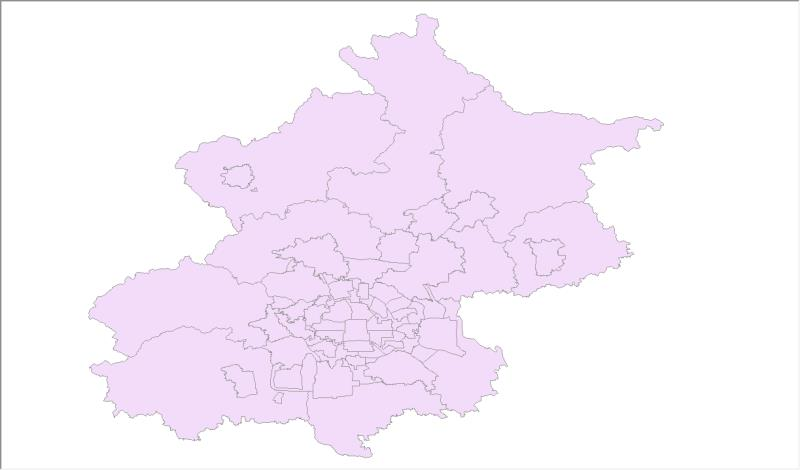
\includegraphics[width=\linewidth]{./images/big_traffic_zone.jpg}
  	\caption{Big zones}
  \end{subfigure}
  \begin{subfigure}[b]{.3\textwidth}
  	\centering
  	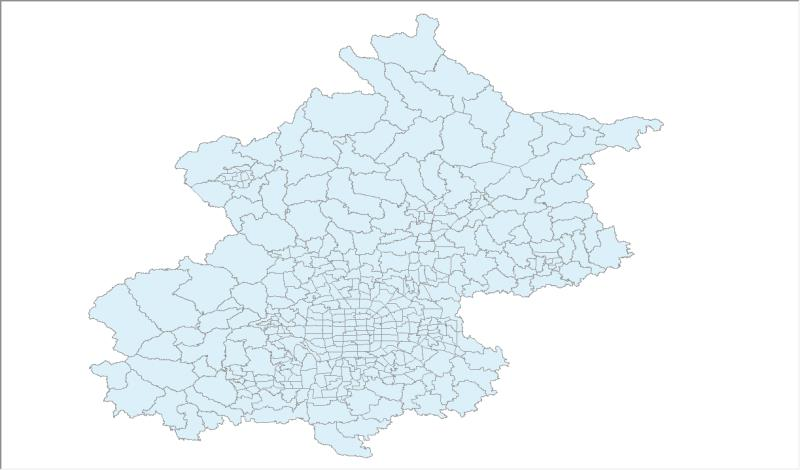
\includegraphics[width=\linewidth]{./images/middle_traffic_zone.jpg}
  	\caption{Middle zones}
  \end{subfigure}
  \begin{subfigure}[b]{.3\textwidth}
  	\centering
  	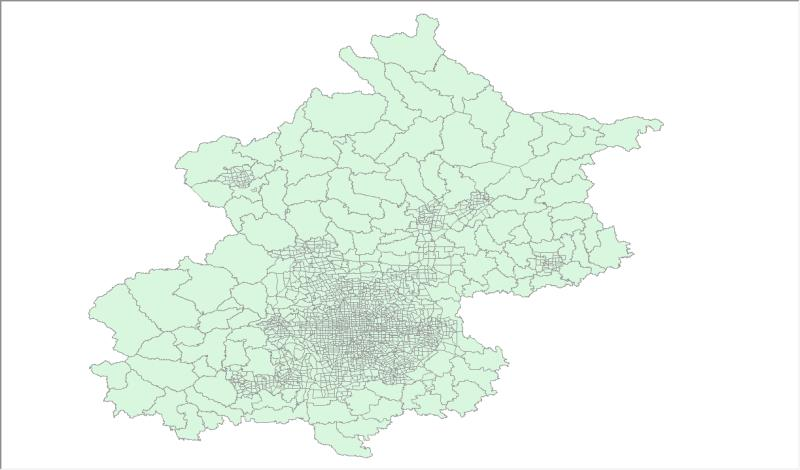
\includegraphics[width=\linewidth]{./images/small_traffic_zone.jpg}
  	\caption{Small zones}
  \end{subfigure}
  \caption{Traffic zone division}
  	\label{fig:data/traffic_zones}
\end{figure}

\begin{figure}
  \centering
  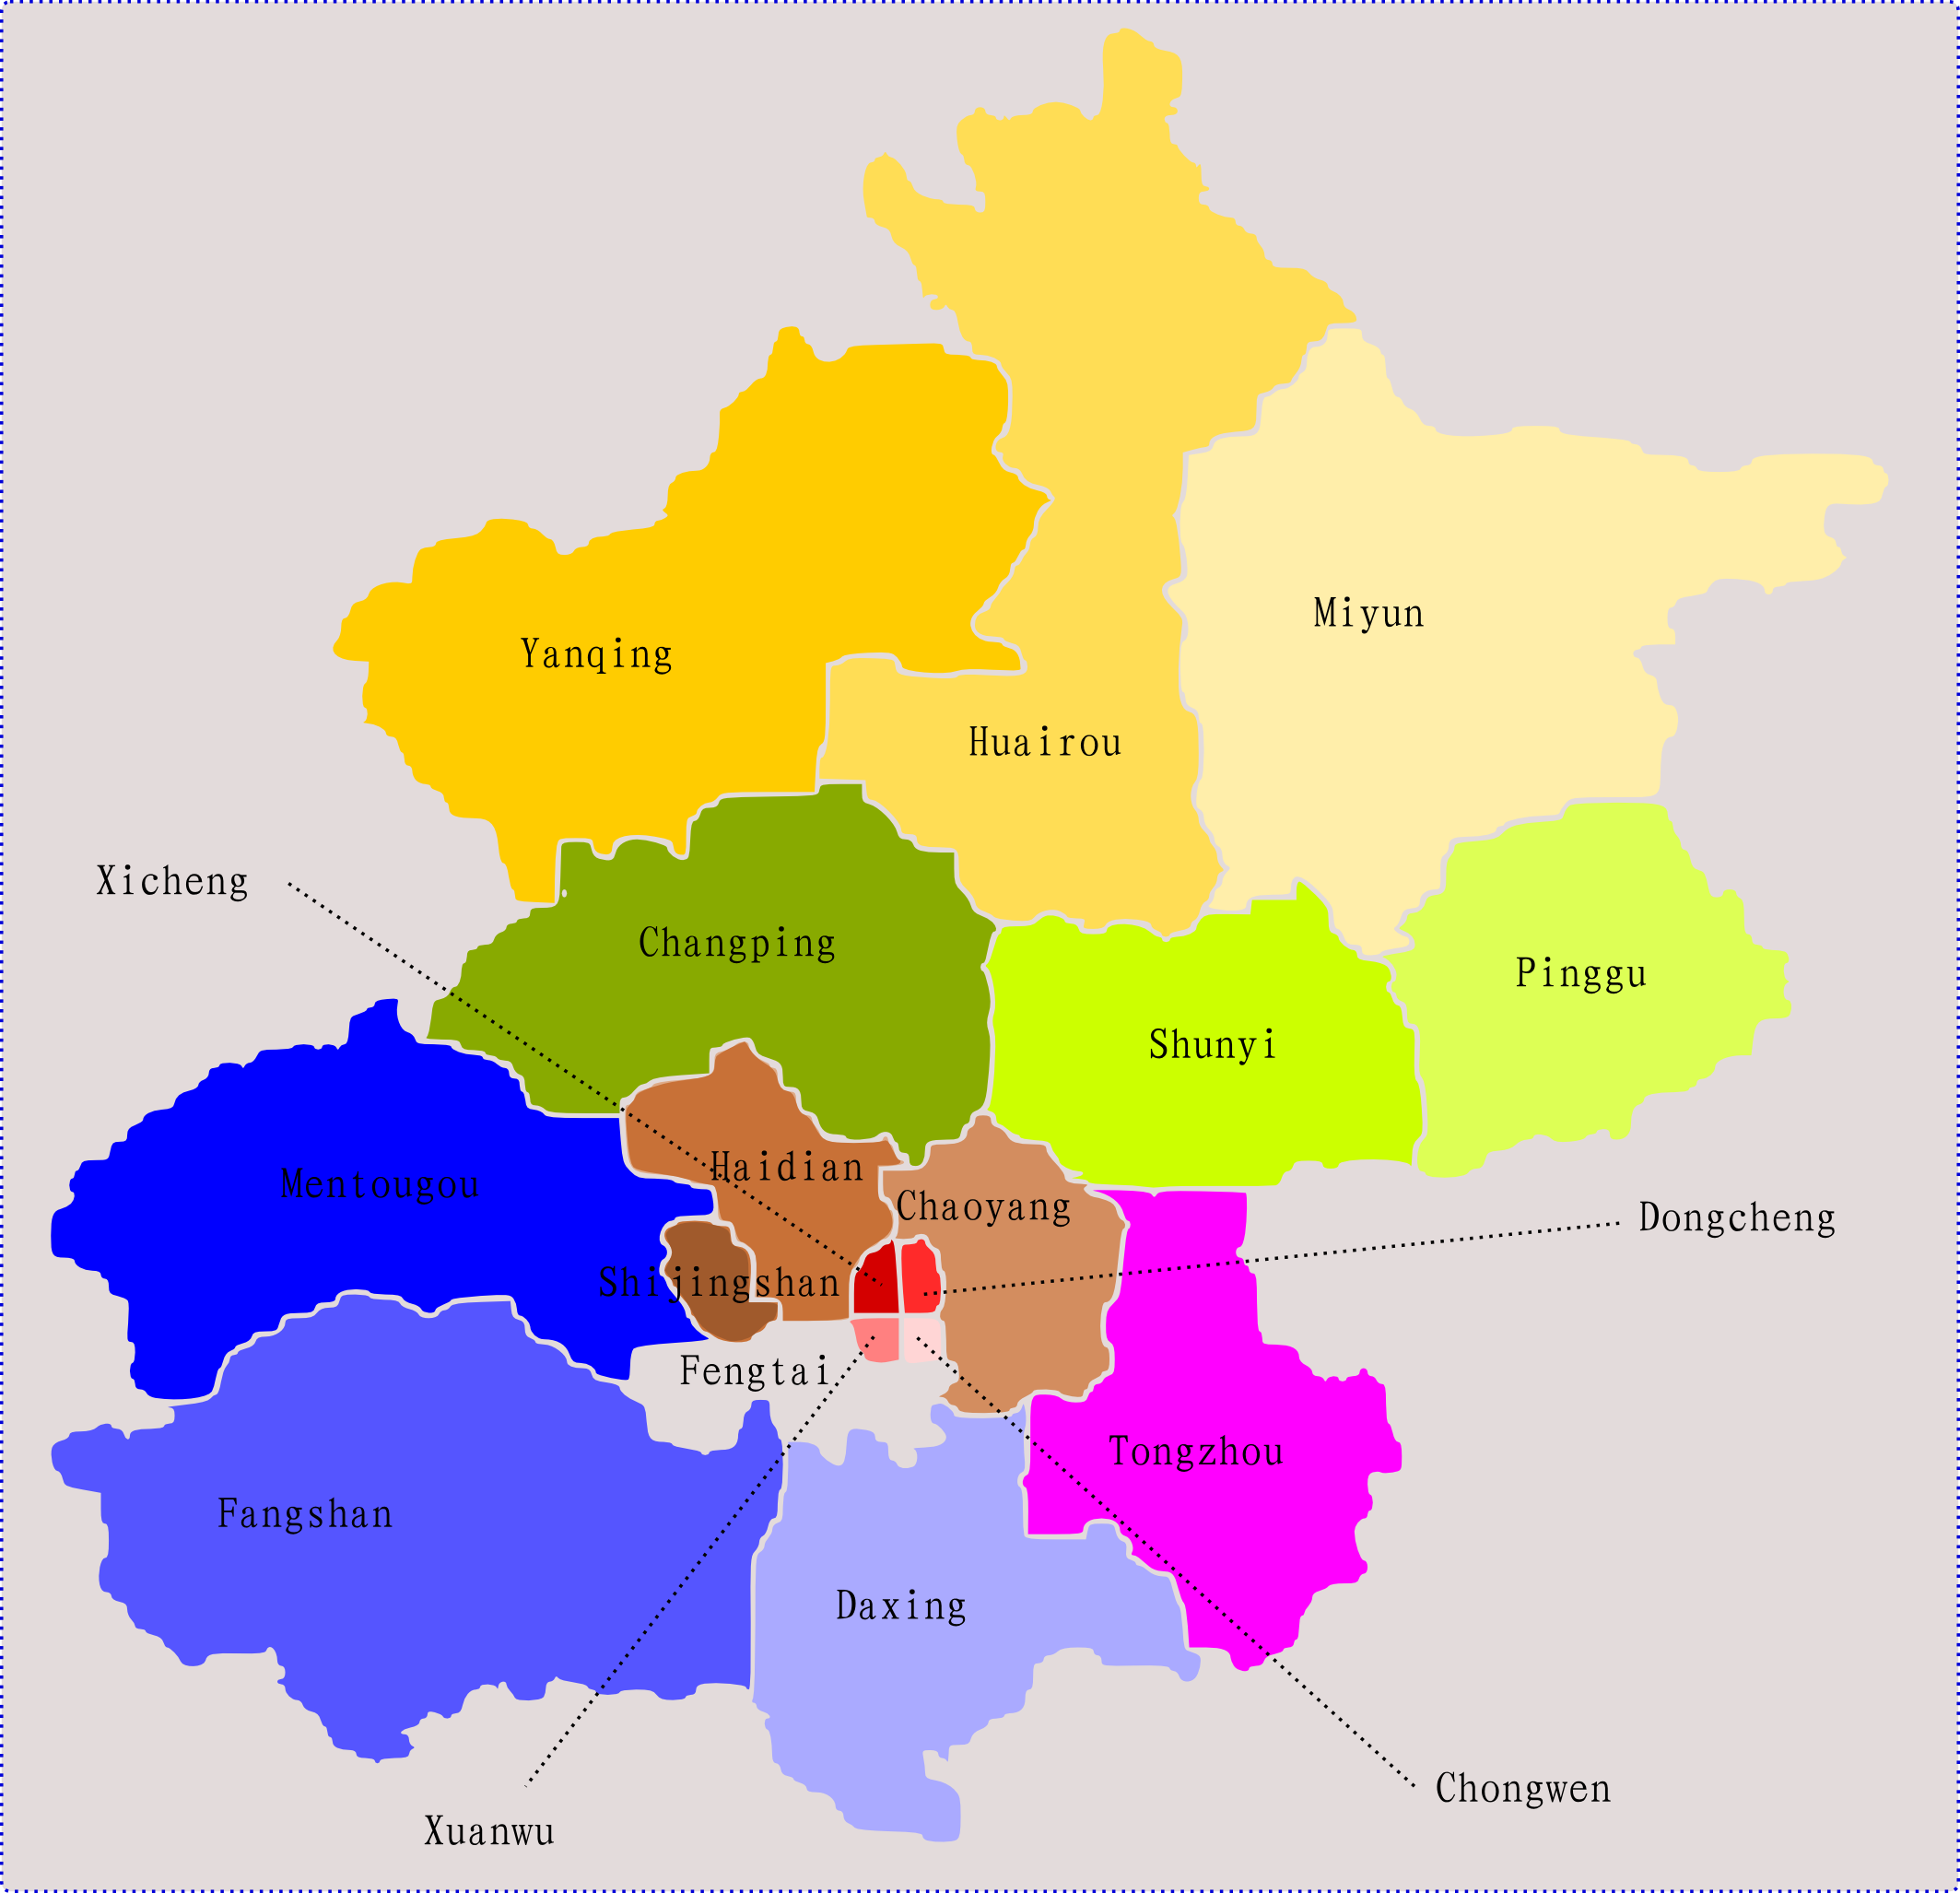
\includegraphics[width=.8\linewidth]{./images/beijing_18areas.png}
  \caption{Beijing's Districts and its Counties}
  \label{fig:data/18areas}
\end{figure}

Every day, more than 13 million records are collected, with approximately 5 million corresponding to subway trips, 8 million corresponding to bus trips, and 100,000 corresponding to bicycle trips. All records corresponding to one day are saved in a single csv file. 

In this project we examine one month worth of data, corresponding to November 2015. The month of November is chosen because it does not overlap with holidays and has a relatively stable weather, hence diminishing the variance between bicycle and bus/subway traveler preferences. As a result, the data to be analyzed is divided into 30 csv files, requiring a total storage space of 53GB.

\subsubsection{Special considerations}
The previous description corresponds to the data as delivered by the TOCC. As such, it is the result from processing the raw records at the collecting phase. Some special considerations concerning this processing are explained below:

\begin{description}%[align=right,labelwidth=2cm]
\item[Travel distance by bike:] Since bicycles do not have predefined routes, the distance cannot be directly recorded. However, it is inferred by using the travel time and a static average speed for cyclists. 

\item[Subway transfer:] Transfers between subways lines of the same operator cannot be tracked since a single check-in gives access to the traveler to all the subway network. In order to infer the transfer detail, the A* algorithm is used to calculate the most likely transfer sequence, given the boarding and alighting stations. 
Furthermore, similarly to the bicycle missing information, the transfer time inside the subway system cannot be directly recorded. Using a static average walking speed and the known distance in transfer stations, the transfer time is calculated. 

\item[Transfer information:] The path link and transfer number fields are extracted from the transfer detail field. Similarly, the transfer average time is calculated from the transfer total time and transfer number fields. 
\end{description}


\subsubsection{Labeled and unlabeled data}

\begin{figure}[h]
  \centering
  \includegraphics[width=.6\linewidth]{"./images/unlabeled data"} %TODO update image
  \caption{Relation between labeled and unlabeled data.}
  \label{fig:method/unlabeled}
\end{figure}


\begin{description}%[align=right,labelwidth=2cm]
\item[Commuter classification:]
Classification is a supervised learning task, where every training data sample requires an associated label determining its true class. In case of commuter classification, this translates to having smart card codes associated with either a "commuter" or "non-commuter" label. Such data is expensive to obtain and limited in principle, since it obtained by asking public transit users directly if they are commuters or not. Thus, in general, annotated data is not available, and labeling new records falls beyond the scope of this project. 

As a solution for the above, we take advantage of the dataset used by Tu\cite{tu2016impact}. This dataset corresponds to trip records performed during a week in January 2015, and it contains labels for 978 smart cards, collected and validated via surveys. The original dataset distribution is composed by:

\begin{itemize}
\item 6439 records of 481 commuters
\item 1628 records of 497 non-commuters
\end{itemize}

As mentioned in Section \ref{sec:data}, this project considers data corresponding to November 2015. Since both datasets correspond to the same year, we believe the labels to be reasonably relevant for both datasets. As such, in order to construct an extended labeled dataset, we take the 978 labeled smart card codes from Tu's dataset, and search for their corresponding records in our dataset. As shown in Figure \ref{fig:method/unlabeled}, a great disadvatage of this is that it tremendously reduces the size of the dataset to less than 1\% of its original size. 

The reduced labeled dataset is used for Part I (Section \ref{sec:partI}) and Part II (Section \ref{sec:partII}) of this project. 

\item[Behavior clustering:]
Clustering, being an unsupervised learning task, does not require labels. Therefore, for this task we are able to use the full dataset. Though rich in its contents, this poses some computational challenges which will be further explained in Section \ref{sec:partI}. %TODO section of DAS5
\end{description}

\subsection{Spatio-temporal representation}
\label{sec:structure}
% 3D locality, channels, bins
One of the main contribution of this project is the novel representation of public transit travel behavior. We consider that the travel behavior of a public transit user is composed by a) the distribution of trips over time, and b) the spatial, temporal and general attributes of each of the trips. 

On the one hand, the distribution of trips over time is a complex continuous distribution. However, according to the Transportation domain standard, it can be approximated in a discrete manner. For this purpose, we divide each day into one hour bins. Then, we consider that each bin can be "occupied" by a trip, or empty if there was no traveling at that moment. 

On the other hand, each trip possesses different attributes of different nature. Fields like \textit{Travel time} and \textit{Travel distance}, for example, have continuous positive values within a reasonable range specific to the city of Beijing. In contrast, fields like \textit{Traffic areas} and \textit{Ring road}, for example, contain categorical values. Therefore, the information from smart card transactions is processed to extract relevant the attributes. 

We propose a 3 dimensional data structure to contain the monthly travel information of a public transit user. The conceptualization is pictured in Figure \ref{fig:data_mining/3D_structure}.

\begin{figure}[H]
  \centering
  \includegraphics[width=.9\linewidth]{./images/3D_structure.png}
  \caption{Spatio-temporal data structure.}
  \label{fig:data_mining/3D_structure}
\end{figure}

Inspired by Langlois et al. \cite{langlois2016inferring}, the x-y plane of our representation constructs a temporal structure between days of the month and hours of the day. The crucial advantage of this structure lies in its local properties. Similar to the case of Image Processing, in this representation a temporal pixel is simultaneously influenced by what happened in the previous/following hours (y axis), and on the previous/following days (x axis).

%TODO maybe redo image to reflect spatial, temporal and general
As for the z axis, each layer contains a trip attribute. In Figure \ref{fig:data_mining/3D_structure} boarding spatial attributes are portrayed in green, alighting spatial attributes are portrayed in red, and other types of general attributes (such as travel time, travel distance, transfer number, transfer total time, etc) are portrayed in yellow. 

Therefore, each temporal pixel may contain a trip feature vector, which expands several layers deep. Considering that even regular public transport users do not usually perform more than 6 trips a day, the proposed representation is sparse, since only a few time pixels are populated with trips.  


\subsection{Dimensionality reduction}
The proposed representation is directly proportional to the number of attributes used to describe a trip. As it is explain in Section \ref{sec:attributes}, we extract 26 attributes in a trip. Considering we have 30 days worth of data, and 24 hourly time bins in a day, this leads to $24 \times 30 \times 26 = 18,790$ temporal pixels to represent one user. Given the high dimensionality and the sparsity of the structure, we need perform dimensionality reduction in order to avoid the typicl effects of the curse of dimensionality. 

\subsubsection{Feature selection}
One of the simplest ways for reducing the number of attributes in a dataset is to perform feature selection. This technique consists of evaluating each feature's influence in making predictions or classifying samples. The strongest features are then selected to be part of the final dataset, while the least informative or redundant features are disregarded. 

When performing feature selection, there are two main choices to be made: the amount of features to be kept and the approaches to evaluate each feature. In this project, the first aspect is tackled using the \textit{Best k} algorithm, which fixes the amount of features to be kept to \textit{k}, regardless of the initial number of features present in the data. The second aspect is tackled via an assortment of algorithms, from statistical tests -such as correlation tests, and ANOVA f-test-, machine learning techniques -such as Trees classifiers-, to domain knowledge from Transportation domain specialists. 

\subsubsection{Feature extraction}
An alternative way of performing dimensionality reduction is by mapping high dimensional spaces to a low dimensional space. Though in most cases the mapping causes some loss of information, there exists mathematical transformations optimized for reducing the loss. Two of the most common techniques to do so are performing single value decomposition, as used by PCA, or work under the Universal Approximation Aroblem, as neural networks. 

In this project, we perform the mapping through an autoncoder. Autoencoders follow the principles of neural networks, and focus on the task of encoding and decoding an image minimizing the loss but not abstracting the noise. As a network, autoencoders may become as complex as needed, allowing for any number of layers and any types of activation functions. 

Taking advantage of the local properties of the proposed representation, we decide to apply stacked convolutional filters followed by a final fully conencted layer that outputs features of a more manageable dimensionality. The end result will be used as features for clustering commuters in Part III (Section \ref{sec:partIII}) of this project. 

%TODO re read starting from here

\subsection{Pattern recognition}

\subsubsection{Ensemble models for classification}
There is a large variety of algorithms for performing classification tasks. Each algorithm may focus on different samples when learning the task, and so has strengths and weaknesses different from one another. 

Ensemble models explore the idea of combining several non-correlated prediction methods that might correct each other in order to reach a better classification accuracy. Furthermore, ensemble models are robust and modular. Therefore, starting from a few weak classifiers, assembled via aggregation methods, the model can grow larger or more complex as needed.

This project constructs an ensemble model for classifying commuters. As proven by Tu \cite{tu2016impact}, weak classifiers like a Support Vector Machines (SVM) is sufficient to identify commuting behavior up to a 94\% accuracy. Aiming to increase accuracy, but aiming to avoid overfitting, this project extends Tu's model with other similar weak classifiers such as decision trees, a Bayesian classifier, a Gaussian process, and a multilayer perceptron. Bagging will be used to ensemble their predictions. %TODO bagging or majority vote?

\subsubsection{Clustering} 
For the third part of this project we perform behavior clustering. To this end, we apply the \textit{K means} algorithm on the low dimensional features extracted by the autoencoder. \textit{Kmeans} is the standard algorithm used in the Transportation domain, and it consistently achieves satisfactory results. 

\subsection{Big Data considerations}
The amount of data gathered for this project require specific computational resources. While programming the tasks, measures are taken to optimize the code. For example, the code is written in modules that work with one day file at the time, and save checkpoints at every relevant step. Additionally, the code is compatible with cluster computing and SLUM jobs are created for its processing.

Furthermore, parallel computing techniques are implemented wherever the whole dataset goes into memory. As shown in Figure \ref{fig:bigdata/parallel}, the time required for applying a single filter reduces drastically if the number of tasks equals the number of cores in the machine used. 

\begin{figure}[H]
  \centering
  \includegraphics[width=.6\linewidth]{"./images/Parallel implementation"}
  \caption{Number of tasks.}
  \label{fig:bigdata/parallel}
\end{figure}

The computational resources are provided by Vrije Universiteit Amsterdam. The results of this project are obtained by using DAS5 (The Distributed ASCI Supercomputer 5) \cite{bal2016medium}. 

\newpage
\section{Data preparation and preprocessing}
\label{sec:partI}
The data acquired for this project corresponds to November 2015. However, due to defective collection methods, the data from November 9 to November 14 is not available. This may have significant effects in the results of the project, as discussed in Section \ref{sec:conclusion}

\subsection{Cleaning}
As first step for preparing the data for its mining, we eliminate faulty records. To this end, we apply the following four filters:

\begin{enumerate}
\item Eliminate records with empty fields: \~10.93\% records eliminated
\item Eliminate records with incomplete travel details: \~1.58\% records eliminated
\item Eliminate records with travel time $<= 0$: <0.01\% records eliminated
\item Eliminate records with travel distance $<= 0$: \~9.82\% records eliminated
\end{enumerate}

\begin{figure}[H]
  \centering
  \includegraphics[width=.6\linewidth]{"./images/faulty data"} %TODO run on whole
  \caption{Reasons for eliminating records.}
  \label{fig:preprocessing/faulty}
\end{figure}

The percentage of data eliminated by each filter is shown in Figure \ref{fig:preprocessing/faulty}. We see removing faulty data reduces the dataset to \~77.66\% of its original size. 

\begin{figure}[H]
  \centering
  \includegraphics[width=.6\linewidth]{"./images/Number of trips_hist"}
  \caption{Number of trips distribution. 2500 record sample.}
  \label{fig:preprocessing/num_trips}
\end{figure}

Figure \ref{fig:preprocessing/num_trips} shows the distribution of number of days in a single day. Its shows that most people perform two trips per day. %TODO find better place to put this 

\subsection{Extraction}

\subsubsection{Time bins}
Regardless of its criticism, using hourly time bins is standard practice in the field and has proven sufficient to examine temporal data \cite{langlois2016inferring} \cite{ma2017understanding} \cite{morency2007measuring}. Therefore, in this project we follow the same technique and extract the hour of the start and end of each trip.

\begin{figure}[H]
  \centering
  \includegraphics[width=.6\linewidth]{"./images/Hour of trip_hist"}
  \caption{Distribution of start/end hours for trips. 2500 records sample.}
  \label{fig:preprocessing/start_end_hour}%TODO rerun in general, or one weekday and one weekend
\end{figure}

From Figure \ref{fig:preprocessing/start_end_hour}, we note that our data follows the expected distribution for the domain, showing clear morning and evening peaks. Furthermore, we note that boarding and alighting patterns during the peaks hours are shifted by one hour. %TODO revise this

\subsubsection{Trip parsing} 
\label{sec:tripParsing}
The trip details obtained from the records are in Chinese, with descriptors containing a combination of numbers and text. In order to extract boarding/alighting route features, the descriptors must be parsed. 

We parse the trip details using a combination of two techniques: regular expressions and the construction of an ID vocabulary. 

\textbf{Regular expressions}

Since a trip may include transfers, we define a trip to be composed of one or many rides. Each ride is carried out in a single travel mode. 

In order to obtain the elements of each ride we look at the descriptor pattern according to its travel mode.

    \begin{align*}
    BIKE &= (bike.STOP-STOP) \\
    SUBWAY &= (subway.LINE:STOP-LINE:STOP) \\
    BUS &= (bus.ROUTE(DIRECTION-DIRECTION):STOP \\
    &-ROUTE(DIRECTION-DIRECTION):STOP)
	\end{align*}
	
where the upper-case text corresponds to placeholders for ride elements, the lower-case text corresponds to the English translation of the descriptor in Chinese, and the punctuation (parentheses, dots, colons and dashes) correspond to separators between ride elements.

Unifying the mode-specific patterns, we describe a ride and a trip using regular expressions:
    
	\begin{align*}	        
    RIDE &= (MODE.[LINE/ROUTE:]?STOP-[LINE/ROUTE:]?STOP) \\
    TRIP &= RIDE[->RIDE]? 
	\end{align*}    
	
where elements surrounded by squared brackets and followed by a question mark (e.g. $[ELEMENT]?$) correspond to optional elements. We note that when parsing bus details, we disregard the route direction. This decision is motivated to fit both subway lines and bus routes to a single pattern, noting that the direction of the route does not affect the path of the route itself.

\textbf{ID Vocabulary}

Once the elements of a trip are extracted, they must be labeled by unique numerical IDs. These IDs are not available from the TOCC, we labeled them using our own system. Two different vocabularies are created, the first one for subway lines/bus routes, and the second one for stops. 

Usually, bus routes are identified by a number. However, in Beijing a single bus route number can be associated to different paths. For example, night buses, express buses and other special cases of a bus route may follow different paths even if they are described with the same number. For this reason we create a vocabulary with all unique parsed routes according to their full description and not only their number.  

Examples of clean routes are shown in Figure \ref{fig:preprocessing/parsed_routes}. %TODO chinese latex!

\begin{figure}[H]
  \centering
  \begin{subfigure}[b]{.8\textwidth}
  	\centering
  	\includegraphics[width=\linewidth]{./images/details_bus.png}
  	\caption{Bus route}
  \end{subfigure}
  \begin{subfigure}[b]{.8\textwidth}
  	\centering
  	\includegraphics[width=\linewidth]{./images/details_subway.png}
  	\caption{Subway route}
  \end{subfigure}
    \begin{subfigure}[b]{.8\textwidth}
  	\centering
  	\includegraphics[width=\linewidth]{./images/details_bike.png}
  	\caption{Bike route}
  \end{subfigure}
  \caption{Examples for parsed and tokenized trip details.}
  	\label{fig:preprocessing/parsed_routes}
\end{figure}

\subsubsection{Calendar-based information} %TODO rephrase
We also extract two attributes from the date of the trip. Day is a number of on the month, from 1 to 30. Weekday is a number from 1 to 7 corresponding to the day of the week, starting on Monday.

\subsection{Data patching}
\label{sec:patching}
We note that the number of transfers and the path link fields of some records do not correspond to the information in their trip details. According to domain expert PhD. Tu Qiang, this must be recalculated \cite{tommy}. 

\begin{figure}[H]
  \centering
  \includegraphics[width=.6\linewidth]{"./images/Number of transfers_hist"}
  \caption{Transfer number distribution before and after recalculation.}
  \label{fig:preprocessing/num_transfers}
\end{figure}

Figure \ref{fig:preprocessing/num_transfers} shows the distribution of the number of transfers per trip before and after patching. The patched distribution shows that most trips are performed without transfers, which is consistent with other studies findings \cite{bhaskar2015passenger}.

\subsection{Standardization} 

\textbf{Continuous values}

In data mining, it is a standard practice to perform whitening. This technique eliminates correlations between features, which is desirable in most cases. However, for the domain of Metropolitan Transportation some of these correlations are highly important and should not be discarded. This is the case of total travel time and distance, as shown in Figure \ref{fig:preprocessing/distance_time_correlation}. For this reason, we choose to only standardize the attribute but keep the correlations. 

\begin{figure}[H]
  \centering
  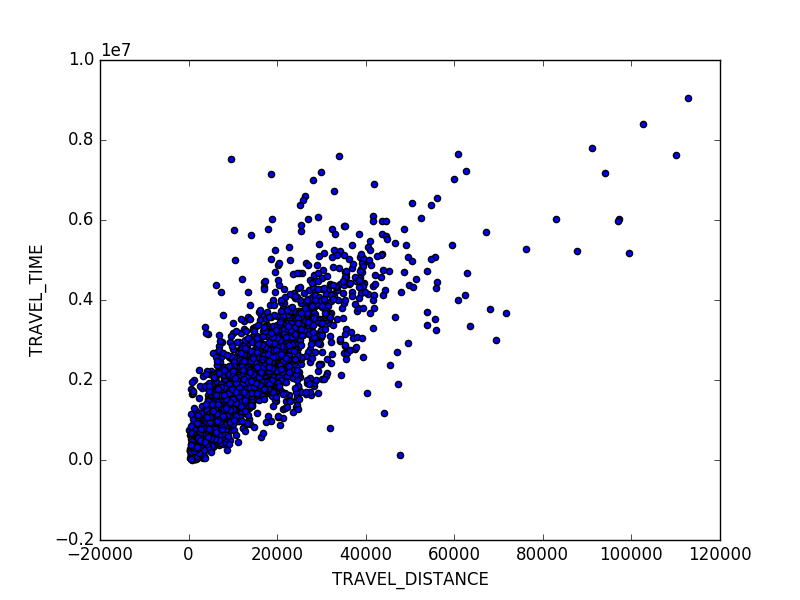
\includegraphics[width=.6\linewidth]{./images/distance_vs_time.png}
  \caption{Travel distance vs travel time. 2500 record sample.}
  \label{fig:preprocessing/distance_time_correlation}
\end{figure}

Travel time, travel distance, total transfer time and average transfer time are standardized by subtracting the mean of each distribution and forcing a unit standard deviation.

\begin{figure}[H]
  \centering
  \begin{subfigure}[b]{.45\textwidth}
  	\centering
  	\includegraphics[width=\linewidth]{"./images/Travel time_hist"}
  	\caption{Original}
  \end{subfigure}
  \begin{subfigure}[b]{.45\textwidth}
  	\centering
  	\includegraphics[width=\linewidth]{"./images/Travel time standardized_hist"}
  	\caption{Standarized}
  \end{subfigure}
  \caption{Time distribution before and after preprocessing. 2500 records sample.}
  	\label{fig:preprocessing/time}
\end{figure}

\begin{figure}[H]
  \centering
  \begin{subfigure}[b]{.45\textwidth}
  	\centering
  	\includegraphics[width=\linewidth]{"./images/Travel distance_hist"}
  	\caption{Original}
  \end{subfigure}
  \begin{subfigure}[b]{.45\textwidth}
  	\centering
  	\includegraphics[width=\linewidth]{"./images/Travel distance standardized_hist"}
  	\caption{Standarized}
  \end{subfigure}
  \caption{Distance distribution before and after preprocessing. 2500 records sample.}
  	\label{fig:preprocessing/distance}
\end{figure}

Figure \ref{fig:preprocessing/time} and \ref{fig:preprocessing/distance} show distributions for travel time and distance. Since the nature of the data prevents negative values (time and distance must be positive), the original distribution is truncated at 0. Standardization maintains the shape of the distribution, but shifts and contracts it to be closer to zero values.

The mean travel time is ~55 minutes, and the mean travel distance is ~10 kilometers.  
 
\begin{figure}[H]
  \centering
  \begin{subfigure}[b]{.45\textwidth}
  	\centering
  	\includegraphics[width=\linewidth]{"./images/Total transfer time_hist"}
  	\caption{Original}
  \end{subfigure}
  \begin{subfigure}[b]{.45\textwidth}
  	\centering
  	\includegraphics[width=\linewidth]{"./images/Total transfer time standardized_hist"}
  	\caption{Standarized}
  \end{subfigure}
  \caption{Total transfer time distribution before and after preprocessing. 2500 records sample.}
  	\label{fig:preprocessing/transfer_time}
\end{figure}

\begin{figure}[H]
  \centering
  \begin{subfigure}[b]{.45\textwidth}
  	\centering
  	\includegraphics[width=\linewidth]{"./images/Average transfer time_hist"}
  	\caption{Original}
  \end{subfigure}
  \begin{subfigure}[b]{.45\textwidth}
  	\centering
  	\includegraphics[width=\linewidth]{"./images/Average transfer time standardized_hist"}
  	\caption{Standarized}
  \end{subfigure}
  \caption{Average transfer time distribution before and after preprocessing. 2500 records sample.}
  	\label{fig:preprocessing/transfer_avg}
\end{figure}

Figure \ref{fig:preprocessing/transfer_time} and \ref{fig:preprocessing/transfer_avg} show that transfer times, both total and average, follow distributions with very long tails. As mentioned before, most trips are performed without transfers, which explains that most of the trips have transfer times equal to zero. %TODO remove top, examine tail

\textbf{Categorical values}

As mentioned in Section \ref{sec:structure}, a trip contains both continuous and categorical attributes. Usually categorical values are to be transformed into one hot encoding. However, in this case that option is not scalable and we do not apply it.


\subsection{Attributes}
\label{sec:attributes}
After the data is preprocessed, we collect 26 attributes that describe a trip. We divide them onto three categories: general attributes, temporal attributes and spatial attributes. 

The general trip attributes are: 

\begin{enumerate}
\item Number of day
\item Weekday
\item Number of trips
\item Travel time
\item Travel distance
\item Number of transfers
\item Transfer total time
\item Transfer average time
\end{enumerate}

The temporal trip attributes are:
 
\begin{enumerate}
\item Start hour
\item End hour
\end{enumerate}

finally, the spatial attributes are:

\begin{enumerate}
\item On/Off District
\item On/Off Small traffic area
\item On/Off Middle traffic area
\item On/Off Big traffic area
\item On/Off Ring road
\item On/Off Mode
\item On/Off Line/Route
\item On/Off Stop
\end{enumerate}

\subsection{User cubes}
%TODO add weekdays of missing dates
Figure \ref{fig:preprocessing/cubes} shows the first slice for a random Commuter and a random Non-commuter


\begin{figure}[H]
  \centering
  \begin{subfigure}[b]{.7\textwidth}
  	\centering
	\includegraphics[width=\linewidth]{"./images/Commuter Day"}
  	\caption{Sample Day slice for random Commuter.}
  \end{subfigure}
  \begin{subfigure}[b]{.7\textwidth}
  	\centering
	\includegraphics[width=\linewidth]{"./images/Non-commuter Day"}
  	\caption{Sample Day slice for random Non-commuter.}
  \end{subfigure}
  \caption{Sample cube slices.}
  	\label{fig:preprocessing/cubes} %TODO crop
\end{figure}

For the case of the Commuter, we identify a pattern between the 15th and 20th of November. We observe several trips at 6:am and 5:00pm suggesting a typical working schedule. The Non-commuter, in contrast, has an irregular distribution of trips. 

It is important to note that, as mentioned before, the data between November 9th and November 14th is missing. Thus, both cases show a gap in records during these days. However, we note that the gaps are not restricted to these days, and that the behavior is very irregular, even for the case labeled as commuter. 


\newpage
\section{Commuters identification}
\label{sec:partII}

\subsection{Attributes correlation}

\begin{figure}[H]
  \centering
  \includegraphics[width=.9\linewidth]{"./images/General correlation"}
  \caption{Attributes correlation to each other and to label.}
  \label{fig:classification/correlation}
\end{figure}

\textbf{General}

Travel time and travel distance are highly correlated. This is due to the lack of express trips available in the public transit. (example, train stations within Amsterdam that are 1 hour away by bus or 10 minutes away by train)

Transfer average and total time are also highly correlated. As examined in Section \ref{sec:patching}, most trips are have few transfers. 

\textbf{Temporal}

Start and end hour are almost identical. Explained by the fact that most trips are completed within the hour. 

\textbf{Spatial}

Boarding attributes share a stronger connection among themselves than with alighting attributes. Furthermore, traffic areas are hierarchical, thus having a high correlation. Ring road and traffic areas maintain a similar relationship, thus correlating strongly. Line and stops are also strongly related. 

\subsection{Feature selection}
From the correlation matrix we note that some attributes are redundant. Hence, feature selection can help to disregard those which are the least informative. 


We evaluate each attribute via its correlation to the true class label, its importance according to an ExtraTrees classifier, its ANOVA f-value, and the jugdment of usefulness according to domain expert PhD. Liang Qu. Initially, a Chi Squared test was also performed, but was abandoned since it had significant bias in favor of continuous attributes over categorical attributes. 

Each method's scores are normalized to sum up to 1. Then, we aggregate them and calculate the final score. The results are shown in Figure \ref{fig:classification/scores}. 

\begin{figure}[H]
  \centering
  \includegraphics[width=.9\linewidth]{"./images/scores"}
  \caption{Attributes scores.}
  \label{fig:classification/scores}
\end{figure}

For selection, we take a fixed amount of attributes from each category, in order to maintain a balanced set. From the \textit{General attributes}, we select the best 3: Number of trips, Weekday, and Travel time. From the \textit{Temporal attributes} we decide to keep them all, since it is a small set. Thus, we select the best 2: Start hour and End hour. 

For the \textit{Spatial attributes} selection, we design a system for pair selection, meaning that if an attribute is selected, its boarding/alighting counterpart is also selected. As such, we select the best 2: On/Off mode, and On/Off line. 

A final set of 9 features is created, resulting in \~66\% reduction. Finally, the cube slices corresponding to the selected features are kept in the user cubes, and the rest disregarded. The cubes are flatten in order for them to be fed into different weak classifiers. 

\subsection{Model}
As suggested by Tu \cite{tu2016impact} results, the data is almost linearly separable thus simple classifiers such as decision trees may suffice.

We train an SVM, a random forest, a perceptron, a Gaussian Process, and a Bayesian net as weak individual classifiers. Other out of the box ensemble models are trained such as AdaBoost using decision trees. 
 
The six classifiers are evaluated, and the best 4 are kept for ensemble. The final class is calculated using a majority vote rule. 


\subsection{Experiments}
The classifiers performance is reported by its accuracy (True positives rate) on two experiments: one run on a single train/test division of the dataset, and b) average of cross validation over 5 folds. 

\centering %TODO make table pretty
\begin{tabular}{|c|c|c|}
\textbf{Classifier} & \textbf{Single run accuracy} & \textbf{Cross validation accuracy} \\
SVM & 88\% & 70\% (+/- 14)\\
Gaussian process & 78\% & 45\% (+/- 9)\\
Perceptron & 87\% & 72\% (+/- 18)\\
Random Forest & 88\% & 71\% (+/- 8)\\
Adaboost of decision trees & 86\% & 68\% (+/- 12)\\
\end{tabular}

\begin{figure}[H]
  \centering
  \includegraphics[width=.9\linewidth]{"./images/SVM_Heatmap"}
  \caption{SVM confusion matrix.}
  \label{fig:classification/svm_confusion}
\end{figure}

\begin{figure}[H]
  \centering
  \includegraphics[width=.9\linewidth]{"./images/Random forest_Heatmap"}
  \caption{Random forest confusion matrix.}
  \label{fig:classification/rf_confusion}
\end{figure}


\begin{figure}[H]
  \centering
  \includegraphics[width=.9\linewidth]{"./images/AdaBoost of decision trees_Heatmap"}
  \caption{Random forest confusion matrix.}
  \label{fig:classification/adb_confusion}
\end{figure}


\subsection{Discussion}
Random Forests deal well with categorical information. Adaboost deals well with missing information.


\begin{figure}[H]
  \centering
  \includegraphics[width=.9\linewidth]{"./images/Selected features"}
  \caption{Visualization of samples and their labels after feature selection.}
  \label{fig:classification/tsne}
\end{figure}

Figure \ref{fig:classification/tsne} shows the data samples by class, represented on its lower dimensional space (after feature selection). It is clear that the classes are not linearly separable, contrary what was expected as suggested by Tu. 

Therefore, the most likely explanation for the classifiers performance is overfitting. 


\newpage
\section{Commuters clustering}
\label{sec:partIII}

\subsection{Feature extraction}
The features to be fed into the clustering algorithms are obtained by dimensionality reduction. As mentioned before, convolutional filters can exploit local information.

\subsubsection{Convolutional filters}
In order to examine weekly patterns, our the first layer of convolutional filters will have an x dimension of 7 with a stride of 7. Assuming that only the hour previous and after a trip affects the trip, the filter will have a y dimension of 3 with a stride of 1. We do not perform padding, since this would have significant implications in the travel behavior of the user. 

Following this formula:

\begin{align*}
	output = \frac{input - filter}{stride} +1
\end{align*}

We find that the output size after the first convolution is $4 \times 22$. Considering 15 features, this reduces the dimensionality to $4 \times 22 \times 15 = 1320$

Goal is to have a $ 4 \times 3 \times 3 = 36$ structure

\technicalDoubt{what about depth? can I have a filter that is 8 units deep, with 8 stride (features are divided as 8 spatial boarding, 8 spatial alighting and 8 transfer related)? How could this be applied?}

\subsubsection{Autoencoder}
A neural network is constructed to apply the convolutional filter. After the convolution layer, ReLU is applied as activation function. 

TSNE results 

\subsection{Clustering}
Tuning via DB-index

Evaluation

\subsection{Cluster analysis}

\subsection{Discussion}


\newpage
\section{Conclusion and future work}
\label{sec:conclusion}

Faulty data. Missing data from 9 to 16. Gap in between.

Zero values such as end hour, zero transfers and others. Same effect as "empty" bin. 

Overlapping trips. So far one trip per bin/hour. Possible solutions are to concatenate.

Standardization by day.

Selection over trip -> label. 

\newpage
\bibliography{mybib}{}
\bibliographystyle{plain}

\end{document}
